\documentclass[a4paper,abntfigtabnum,noindentfirst]{abnt}
\usepackage[brazil]{babel}
\usepackage[utf8]{inputenc}
\usepackage{graphicx}
\usepackage[alf]{abntcite}

\titulo{Behaviour-Driven Development}
\autor{Rodrigo Soares Manhães\\
\small Instituto Federal Fluminense\\
\small \texttt{rmanhaes@iff.edu.br}\\
}
\date{12 de março de 2010}

\begin{document}
\maketitle

\chapter*{Behaviour-Driven Development}

Behaviour-Driven Development (BDD) é uma técnica de desenvolvimento de software cuja amplitude se estende às atividades de levantamento de requisitos, \textit{design}, documentação e verificação e validação, tratando-as de modo unificado, disciplinado e com foco em qualidade e em entrega rápida de software de valor. BDD encoraja e fornece um ambiente propício à colaboração entre desenvolvedores, setores de qualidade e pessoal de negócios em um projeto de software. BDD foi concebida inicialmente por \citeonline{IntroBDD}, tendo recebido um grande número de contribuições de praticantes ao redor do mundo, principalmente de textos publicados em blogs\footnote{Uma lista com um bom número destes artigos de blogs se encontra no anexo 1.}. \citeonline{RSpecBook} detalham a técnica no contexto de ferramentas BDD para a linguagem Ruby\footnote{http://ruby-lang.org, acesso em 26/02/2009.}, sendo provavelmente o maior conjunto de informações sobre BDD disponível atualmente em uma mesma fonte.

\section*{O ciclo \textit{outside-in}}

Quando se usa BDD, as atividades necessárias ao desenvolvimento de uma funcionalidade são realizadas segundo  um ciclo denominado \textit{outside-in}. O ciclo recebe este nome devido à sequência que deve ser percorrida, que se inicia dos requisitos e da visão do cliente (\textit{outside}) até as entranhas dos artefatos de software (\textit{in}). Este ciclo pode ser explicado em uma série de passos, adaptados de \citeonline{RSpecBook} e comentados:

\begin{enumerate}

\item \textit{Foco em um cenário}\\
Na terminologia de BDD, um cenário é um exemplo de utilização de uma dada funcionalidade. Uma funcionalidade é algo que o software deve oferecer e que possui um valor bem definido para o usuário. Em BDD, o foco dos desenvolvedores deve estar sempre direcionado a um único cenário de uma única funcionalidade por vez. Isto elimina dispersões e mantém o desenvolvedor concentrado na tarefa a ser realizada. Um desenvolvedor utilizando BDD deve encarar um novo cenário como se todos os requisitos do software fossem apenas os cenários já implementados e o atual. Isto é importante para evitar generalizações baseadas em especulações a respeito do que o software possa eventualmente necessitar no futuro, o que aumenta a complexidade do design sem qualquer garantia de que será realmente útil.

\item \textit{Escreva uma especificação para este cenário}\\
BDD possui um pressuposto central segundo o qual nenhuma funcionalidade, no todo em ou parte, é implementada sem a escrita prévia de uma especificação executável. Assim, antes de qualquer atividade de implementação de uma funcionalidade, deve ser escrita de uma especificação, em linguagem natural, de como a funcionalidade deve ser do ponto de vista do cliente. Esta especificação, que chamaremos \textit{especificação do usuário} é executada e, uma vez que ainda não há nada implementado, falha.

\item \textit{Escreva uma especificação de unidade}\\
Para fazer a especificação do usuário executar com sucesso, é necessário implementar algo, seja uma classe, uma função, uma página HTML. É importante perceber que há aqui uma mudança de nível: a especificação do usuário apenas se preocupa com a parte do software visível externamente, mas nada diz a respeito dos diferentes artefatos em código-fonte que comporão o software. Neste ponto é necessário escrever uma nova especificação, desta vez uma \textit{especificação de unidade}, que descreve o funcionamento do artefato (classe, função, página, módulo etc.) que precisa ser implementado para cumprir a especificação do usuário. A especificação de unidade recém-escrita, ao ser executada igualmente falhará, pela simples inexistência da implementação. É importante ressaltar que a especificação de unidade deve ser apenas minimamente suficiente para que a especificação do usuário passe. Quaisquer outras necessidades que se possam prever de antemão devem ser adiadas até que um outro cenário da especificação do usuário as solicite.

\item \textit{Faça a especificação de unidade passar}\\
Neste momento, o artefato de software deve ser implementado de modo a passar na especificação de unidade. A implementação deve ser a mais simples e mínima possível, apenas o estritamente necessário para fazer a especificação passar. BDD, vale lembrar, trabalha orientada ao usuário e à geração de valor para este. Além disto, enquanto código útil é um patrimônio que gera valor, qualquer código criado inutilmente é tempo desperdiçado e, no fim das contas, um passivo, que sem gerar valor algum, aumentará a complexidade geral do software. O uso de técnicas de efetiva garantia de qualidade como BDD, aliado a técnicas modernas de design e boas práticas de programação \cite{CleanCode} \cite{ImplementationPatterns} tornam desnecessária a obsessão com ``estar preparado para as mudanças'' que assolou os programadores e designers em tempos idos.

\item \textit{Refatore}\\
Conforme o item anterior, em BDD todo código deve ser implementado apenas para satisfazer às especificações atuais, sem maiores preocupações em criar facilidades para acomodação de novos requisitos. Estas preocupações normalmente se expressam por meio de pensamentos como ``é melhor fazer desde já esta associação como muitos-para-muitos, pois é muito provável que isto seja necessário no futuro''. É natural que haja este tipo de preocupação, uma vez que é fato conhecido de qualquer desenvolvedor de software que a simplicidade e clareza do \textit{design} tendem a decair no decorrer do tempo. Assim, mudanças são mais simples de serem aplicadas no início do projeto do que em tempos posteriores. Isto se traduz na famosa curva de Boehm, que mostra que o custo das modificações em um projeto de software sobe exponencialmente no decorrer do tempo \cite{Boehm1981}. BDD se utiliza de uma técnica conhecida como refatoração\footnote{``Refatoração'' é a tradução consagrada na literatura em língua pátria, ainda que discutível, do original inglês \textit{refactoring}.}, que consiste em aperfeiçoar o \textit{design} interno de uma aplicação sem qualquer percepção de mudança sob o ponto de vista dos usuários. Na refatoração, o código que foi implementado apenas com o mínimo necessário para fazer a especificação passar deve agora ser reestruturado de modo a se adequar harmoniosamente ao \textit{design} preexistente. Quando se usa BDD, não se faz um \textit{design} prévio detalhado. Ao contrário, o \textit{design} evolui \cite{XP2ndEd} \cite{EmergentDesign} a cada nova especificação implementada, sendo o papel da refatoração manter o \textit{design} sempre da forma desejada. A princípio, o uso de refatorações pode parecer algo temerário, pois seria alterar a estrutura de uma aplicação, abrindo-a à possibilidade da introdução de defeitos. Isto, porém, não ocorre, pois o uso de refatoração é inseparável de uma ampla cobertura de testes automatizados, papel que em BDD cabe às especificações automatizadas. Se qualquer código escrito é precedido por uma especificação que o exija, logo, todo o código da aplicação está coberto por especificações automatizadas, o que dá uma generosa margem de segurança para a melhoria do \textit{design}. \citeonline{Refactoring} explicam detalhadamente o conceito de refatoração e apresenta um extenso catálogo, escrito à moda dos textos sobre patterns, com refatorações comprovadas na prática.\\
\\
Os passos 3 a 5 devem ser repetidos até que todo o cenário passe.

\item \textit{Refatore}\\
Este novo passo de refatoração se deve a uma nova mudança de nível: desta vez em sentido contrário. Da implementação (itens de software) para o requisito (visão do usuário). Neste nível, novas melhorias podem ser introduzidas no design, sempre com o intuito de simplificar e tornar o \textit{design} mais claro, simples e comunicativo.

\end{enumerate}


\section*{Uma linguagem universal para especificação de software}

Em muitos projetos de software, a terminologia e, principalmente, os conceitos utilizados diferem bastante entre os utilizados pelos clientes em seu dia-a-dia, os utilizados pelos desenvolvedores em suas conversas internas e aqueles efetivamente implementados em software. Por vezes, mesmo dentro do software há este tipo de diferenciação, por exemplo, entre a camada de lógica de negócios e a estrutura de persistência subjacente. Estas diferenças e as constantes traduções necessárias para passar de um contexto a outro geram um considerável \textit{overhead} e são um foco de confusão e de introdução de defeitos no software.

Para resolver este problema, \citeonline{DDD} propôs o conceito de \textit{ubiquitous language} (UL), uma visão unificada do software e compartilhada entre os membros da equipe de desenvolvimento e os clientes. Esta visão unificada deve se traduzir tanto nas conversas entre os desenvolvedores entre eles e com os clientes quanto nos conceitos e nomenclaturas adotadas na implementação do software, dos rótulos nas interfaces gráficas aos nomes de campos e tabelas no banco de dados.

BDD se apresenta como uma UL para especificação de software, uma vez que traz uma série de conceitos e um vocabulário bem definido. O módulo básico de BDD é a funcionalidade (no original, \textit{feature}). O conceito de funcionalidade tem estreita ligação com o conceito de \textit{user story} \cite{XP2ndEd} \cite{UserStoriesApplied} e pode na maioria das vezes correlacionar com um caso de uso da UML \cite{UML}\footnote{Uma grande diferença entre um caso de uso e uma \textit{user story} é que esta não é a descrição detalhada de uma funcionalidade do software, mas simplesmente a documentação de um desejo do usuário. Uma funcionalidade (\textit{feature}) em BDD é a especificação detalhada de uma \textit{user story}, vindo daí a semelhança entre casos de uso UML e \textit{features} BDD.  Além disto, são semelhantes no fato de serem instrumentos para coleta e documentação detalhada de requisitos. As semelhanças, porém, param aí, pois as diferenças conceituais, tecnológicas e de aplicação entre as duas são grandes, conforme se verá.}. A \textit{ubiquitous language} de BDD para especificação de funcionalidades é descrita por \citeonline{WhatsInAStory}.

Uma funcionalidade normalmente possui uma descrição que, basicamente, indica quem é o solicitante, como ele descreve a funcionalidade e qual é o valor desta funcionalidade. Para isto são normalmente usadas, respectivamente, as expressões \textit{Como um} (\textit{As a}), \textit{Eu quero} (\textit{I want}) e \textit{Para que} (\textit{So that}, mas também é comum encontrar \textit{In order to}).

Toda funcionalidade possui um ou mais cenários (no original, \textit{scenario}), que são exemplos de casos específicos de utilização da funcionalidade. Cada cenário consiste em um título e uma sequência de passos (no original, \textit{step}) que representam as interações do usuário com o software.

A \textit{ubiquitous language} trazida por BDD prescreve três tipos de passos:
\begin{itemize}

\item \textit{Dado que} (\textit{Given}), que especificam as pré-condições para que ocorra a ação de interesse do cenário;
\item \textit{Quando} (\textit{When}), cuja função é especificar os eventos que devem ocorrer para que o cenário seja executado;
\item \textit{Então} (\textit{Then}), que especificam as expectativas a respeito dos resultados da execução dos eventos do cenário.
\end{itemize}

Um exemplo completo de uma funcionalidade BDD, adaptado de \citeonline{WhatsInAStory}, é mostrado na Figura \ref{exemplo-de-funcionalidade}.

\begin{figure}
	\caption{Exemplo de especificação do usuário}
	\label{exemplo-de-funcionalidade}
	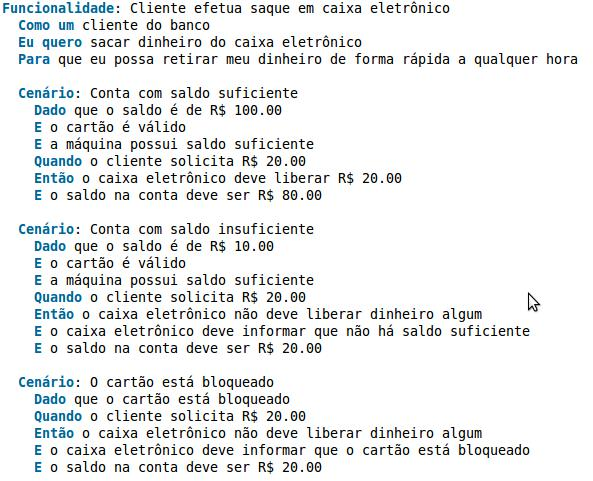
\includegraphics[scale=0.7]{exemplo-de-funcionalidade-bdd}
\end{figure}

Além da terminologia citada, a palavra ``deve'' (\textit{should} no original) também faz parte da \textit{ubiquitous language} de BDD, sendo usada para expressar uma expectativa, sempre nos passos \textit{Então}.

A adoção da nomenclatura de especificações em lugar de testes foi o início da mudança que levou a especificação ao cliente, sendo uma das molas-mestras para a evolução de BDD a partir de TDD, conforme se verá na Seção \ref{HerancaTDD}.

\section*{A Herança de TDD}
\label{HerancaTDD}

BDD tem suas raízes em uma técnica conhecida como Test-Driven Development \cite{TDDByExample}, que, em sua conceituação inicial, equivalia basicamente aos passos 3 a 5 do ciclo BDD apresentado no item 1.1, ou seja, um ciclo de escrever um teste, implementar o mínimo de código necessário para passar no teste e, ao fim, refatorar. Posteriormente, foi desenvolvida sobre TDD a técnica de Acceptance TDD (ATDD), que constituía, basicamente, o ciclo BDD. De fato, os ciclos ATDD em \citeonline{TestDrivenKoskela} e o ciclo BDD em \citeonline{RSpecBook} são conceitualmente os mesmos.

Contudo, TDD possuía alguns problemas em relação à sua nomenclatura e, por consequência, às suas formas de pensar o desenvolvimento de software. TDD, por seu próprio nome, passa a idéia de ser apenas uma técnica de verificação de software, mesmo que muitos autores afirmassem reiteradamente TDD principalmente como uma técnica de \textit{design}, com o bônus de se ganhar a verificação no processo \cite{DrivingSoftwareQualityCrispin} \cite{TDDAstels} \cite{TDDDesignJanzen}. Com ATDD, ainda entram em cena atividades onde a técnica atua o levantamento de requisitos e a validação de software. Ou seja, tudo muito distante de se falar meramente em ``testes''. A nomenclatura de ``testes'' enseja toda sorte de resistências e protestos como ``este código é muito simples, não precisa ser testado'' ou ``Testes? Você está duvidando da minha capacidade?''. Tais questionamentos desaparecem quando se fala em especificação.

Assim, BDD é basicamente uma ATDD com uma \textit{ubiquitous language} adequada. Ou seja, toda a base conceitual e idéias desenvolvidas no mundo (A)TDD como \textit{baby steps}, \textit{features} como especificação de \textit{user stories}, busca pela simplicidade, \textit{design} emergente e tantas outras são completamente válidas para BDD, bastando situar TDD e ATDD nos pontos corretos do ciclo BDD.

Do mesmo modo, a literatura técnica sobre TDD e ATDD é virtualmente de completa validade para estudos em BDD.  \citeonline{TDDByExample} demonstra detalhadamente o uso de TDD em casos concretos, desenvolvendo dois pequenos projetos. \citeonline{TestDrivenKoskela} apresenta Acceptance TDD, aprofundando aspectos teóricos e práticos de TDD e ATDD. \citeonline{xUnitPatterns} traz um extenso catálogo de \textit{patterns} para TDD. \citeonline{GrowingTDD} discutem o uso de TDD no design de software orientado a objetos. Um detalhado exemplo do uso de TDD na implementação da uma funcionalidade, em língua portuguesa, pode ser encontrado em http://www.improveit.com.br/xp/praticas/tdd (acesso em 24/02/2010).

Com relação a estudos sobre os impactos de TDD no desenvolvimento de software, \citeonline{SoftwareArchitectureTDD} conclui que TDD leva a melhoras significativas em métricas como complexidade computacional, acoplamento, volume de testes e cobertura de testes. Posteriormente, \citeonline{TDDDesignJanzen} concluíram que TDD leva um \textit{design} mais orientado a objetos, porém requer profissionais com alto nível de habilidade técnica para obter um \textit{design} com baixo acoplamento. \citeonline{TDDDefectReduction}, em um estudo de caso na indústria, relatam que a aplicação de TDD leva a reduções na densidade de defeitos, com impacto mínimo na produtividade. Contudo, um experimento conduzido por \citeonline{EffectivenessTestFirst} constatou um aumento de produtividade com o uso de TDD, o que foi atribuído a um melhor entendimento das tarefas a serem realizadas, o foco em pequenas partes de funcionalidades de cada vez, a criação de um ambiente de \textit{feedback} constante e aprendizagem e pouco esforço de retrabalho. Os resultados obtidos por \citeonline{TDDDesignJanzen} indicam uma correlação positiva entre TDD e produtividade. Este trabalho também concluiu que os programadores vêem TDD mais positivamente após alguma experiência prática. \citeonline{ArtOfFearlessProgramming} fazem um apanhado de trabalhos sobre TDD e chegam a resultados controversos, relatando, porém, que a maioria dos pesquisadores concorda que TDD leva a um melhor foco nas tarefas sendo realizadas e a aumentos na taxa de cobertura de testes.

\section*{Tópicos adicionais}

\subsection*{Definição de terminado}

Uma das dificuldades mais sutis no desenvolvimento de software é descobrir quando uma funcionalidade está terminada. Na engenharia de software tradicional, com o uso de especificações não executáveis, o término de uma funcionalidade se dá quando o desenvolvedor acredita que o estágio atual da implementação atende às especificações, não havendo uma forma direta e objetiva de verificar isto, o que acaba sendo deixado para ser feito na ``fase'' de testes. Em alguns casos, não há nem mesmo uma especificação que lhe forneça esta informação, tornando esta decisão ainda mais subjetiva.

Quando se cria uma especificação BDD para uma funcionalidade, se tem, automaticamente, uma definição de terminado. Uma funcionalidade está pronta quando passa na especificação, em uma avaliação puramente objetiva, posto que automática. Em BDD, uma especificação do usuário contém intrinsecamente o critério de aceitação da funcionalidade em seus passos Então.


\subsection*{Verificação de regressão}
A engenharia de software tradicionalmente trata a regressão como um problema sem solução ótima. Quando uma nova funcionalidade é adicionada a um software ou este sofre uma manutenção de qualquer tipo, sempre há a possibilidade de que a alteração inadvertidamente inclua falhas no software. Se a implementação dos testes é manual, é na maioria dos casos inviável testar novamente todo o software. O recomendável, nestes casos, é manter um documento com informações de rastreabilidade, de modo a saber que módulos do software são atingidos por uma alteração \cite{EngSoftPressman} \cite{EngSoftSommerville}. Apesar de diminuir bastante a ocorrência de problemas, a criação e manutenção de tais artefatos é complexa e propensa a erros.

Com o uso de técnicas de verificação e validação automatizadas como BDD, é possível simplesmente executar as especificações para todo o software antes de enviar cada alteração ao controle de versões. Caso o tempo dos testes fique alto demais, pode-se particionar por módulo, rodando-se todas as especificações de unidade mas apenas as especificações do usuário relativas ao módulo, uma vez que especificações do usuário, por simular o uso real do software, consomem muito mais tempo para executar. Uma alternativa é tentar otimizar a implementação das especificações de usuário, utilizando, por exemplo, em casos de aplicações web, simuladores de navegador como Webrat\footnote{http://wiki.github.com/brynary/webrat, acesso em 02/03/2010} ou zope.testbrowser\footnote{http://pypi.python.org/pypi/zope.testbrowser, acesso em 02/03/2010} em lugar de ferramentas que usam navegadores reais como Selenium\footnote{http://selenium-rc.seleniumhq.org, acesso em 02/03/2010} ou Watir\footnote{http://watir.com, acesso em 05/03/2010}.

\bibliographystyle{abnt-alf}
\bibliography{referencias}

\end{document}

